\subsection{Workflows}

[CuCo] Corre Configuración de Limpieza de Datos

Workflow para llenar los parámetros necesarios para el dashboard y trabajo óptimo en los procesos de CMI, 
se ejecuta la limpieza respecto a las llaves definidas.

\begin{figure}[H]
    \centering
    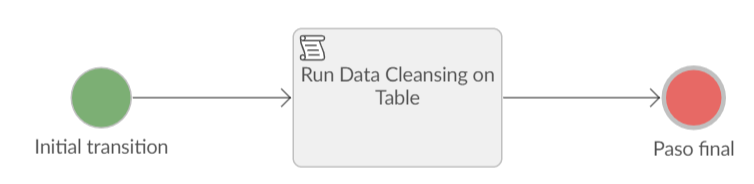
\includegraphics[width=0.8\textwidth]{WorkflowsDashboard/ImgWF/WF01.png}
    \caption{Workflow: Corre Configuración de Limpieza.}
\end{figure}

[CuCo] Importación Genérica de Tabla 

Este modelo hace uso de scripts (procesos técnicos dentro de la herramienta EBX) para ejecutar tareas, las cuales ayudan a reducir una intervención manual en el proceso. Éstas son descritas a continuación:

\begin{itemize}
    \item Eliminar registros: Tarea encargada de borrar todos los registros de la tabla contenedora en TIBCO EBX donde se alojan los datos actuales.

    \item Importar registros: Permite introducir información perteneciente de SAP/COUPA a una tabla contenedor de EBX; para su funcionamiento, se tienen que definir a que tabla se quiere mandar los datos y a que espacio de datos está ligado. Estos datos se configuran previo a su ejecución.
\end{itemize}

\begin{figure}[H]
    \centering
    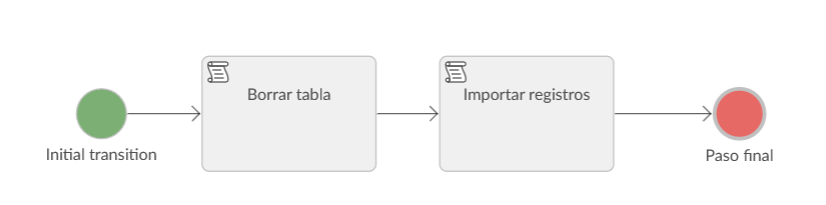
\includegraphics[width=0.8\textwidth]{WorkflowsDashboard/ImgWF/WF02.png}
    \caption{Workflow: Importación Genérica de Tabla.}
\end{figure}

[CuCo] Catálogos - Importación de Data Lake – Maestro V2

Workflow que utiliza el flujo de trabajo de importación genérico comentado anteriormente. Este proceso se encarga de obtener la información relevante para la creación de una cuenta contable.

\begin{figure}[H]
    \centering
    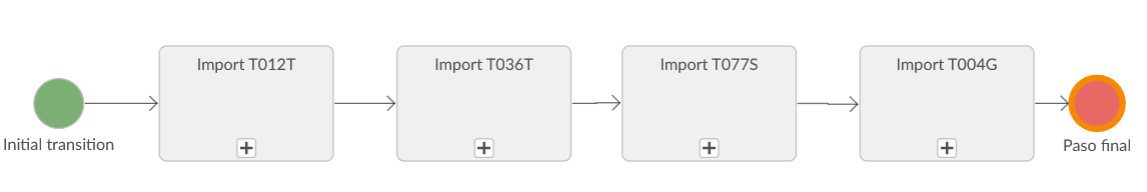
\includegraphics[width=0.8\textwidth]{WorkflowsDashboard/ImgWF/WF03.png}
    \caption{Workflow: Catálogos - Importación de Data Lake – Maestro.}
\end{figure}

\begin{table}[h]
    \centering
    \begin{tabular}{|l|l|}
        \hline
        Nodo de Workflow & Tabla Destino \\
        \hline
        Import T012T & Importación de información para catalogo maestro de Nombre de cuentas bancarias internas. \\   
        \hline
        Import T036T & Importación de información para catalogo maestro de Textos de nivel de planificación. \\  
        \hline
        Import T077S & Importación de información para catalogo maestro de Grupo de cuentas. \\  
        \hline
        Import T004G & Importación de información para catalogo maestro de Grupo de status de campo. \\
        \hline
    \end{tabular}
\end{table}

[CuCO] Catálogos - Importación Data Lake Tablas Master V2

Workflow que utiliza el flujo de trabajo de importación genérico comentado anteriormente. Este proceso se encarga de obtener la información relevante de todas las cuentas contables creadas con anterioridad dentro del Data Lake.

\begin{figure}[H]
    \centering
    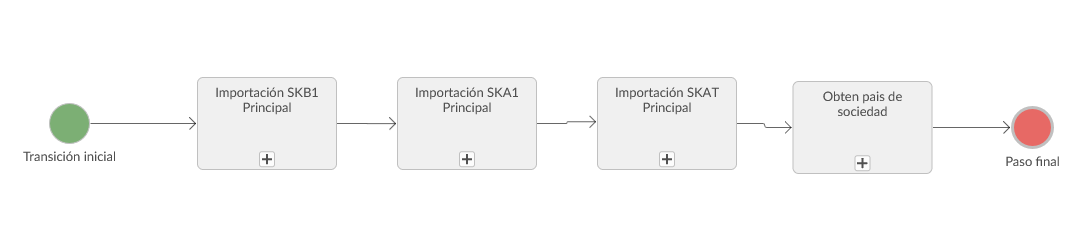
\includegraphics[width=0.8\textwidth]{WorkflowsDashboard/ImgWF/WF04.png}
    \caption{Workflow: Catálogos - Importación Data Lake Tablas Master}
\end{figure}

\begin{table}[h]
    \centering
    \begin{tabular}{|l|l|}
        \hline
        Nodo de Workflow & Tabla Destino \\
        \hline
        Importación SKB1 Principal & Importación de datos para la tabla de Cuenta maestra (sociedad). \\   
        \hline
        Importación SKA1 Principal & Importación de datos para la tabla de Cuenta maestra (Mandante). \\  
        \hline
        Importación SKAT & Importación de datos para la tabla SKAT del espacio de datos de calidad. \\  
        \hline
        Obtén país de sociedad & Proceso auxiliar para obtener el país que esta relacionado a cada sociedad. \\
        \hline
    \end{tabular}
\end{table}

[CuCo] Creación (Nivel PUC) V2

Flujo de trabajo encargado de realizar un proceso de creación de una cuenta contable haciendo uso de catálogos externos para facilitar su creación. Dentro del proceso se hace uso de diversos roles para la creación y revisión del mismo. Además, incluye el envío de dicha cuenta a SAP para la creación de su lado

\begin{figure}[H]
    \centering
    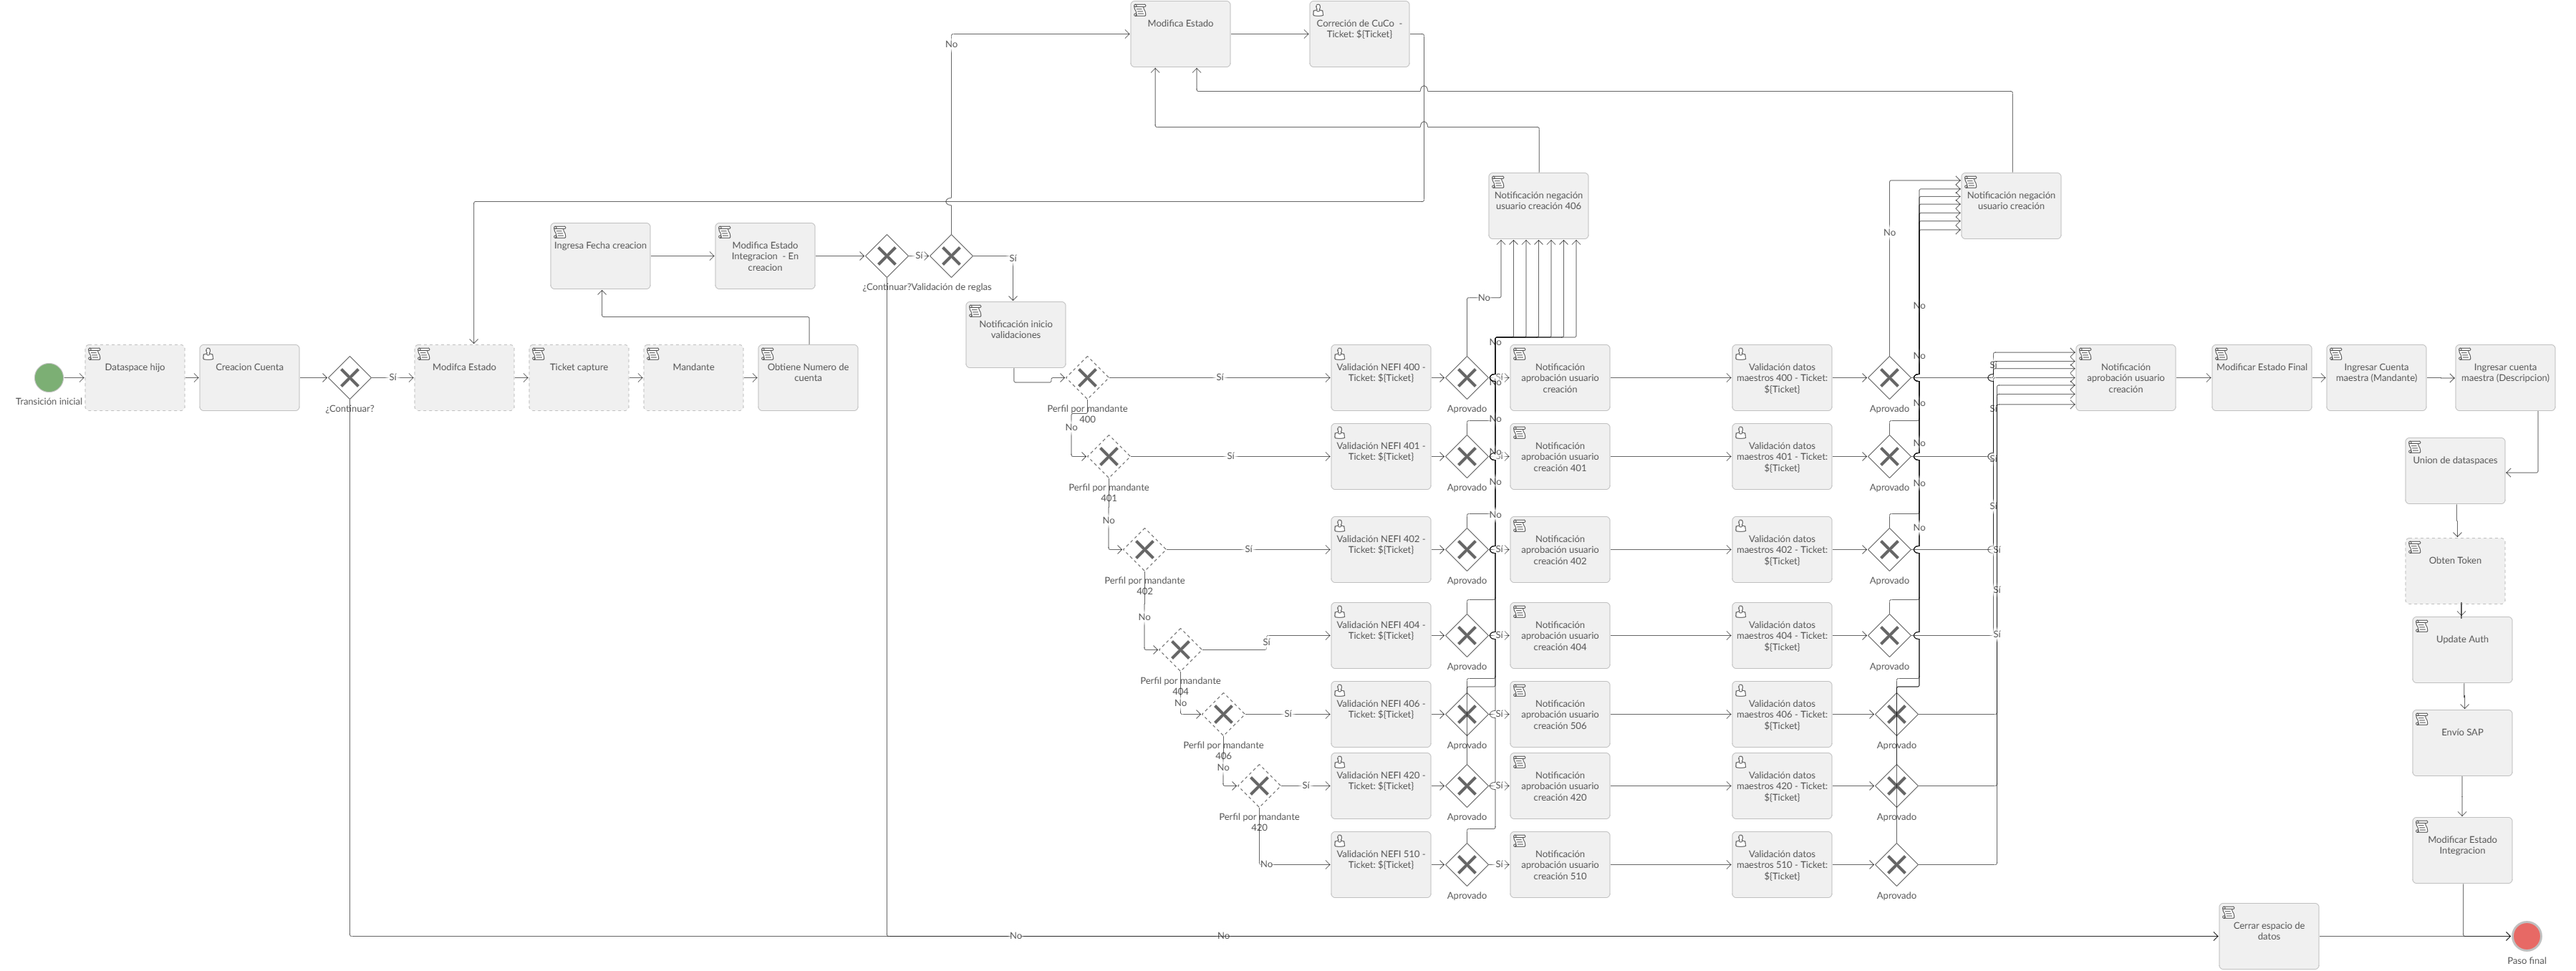
\includegraphics[width=0.8\textwidth]{WorkflowsDashboard/ImgWF/WF05.png}
    \caption{Workflow: Creación V2}
\end{figure}

[CuCo] Expansión de Cuenta V2

Flujo de trabajo a cargo de realizar una ampliación a una cuenta contable. Dentro del proceso incluye las validaciones por cada rol dentro el proceso y el envío de información a SAP.

\begin{figure}[H]
    \centering
    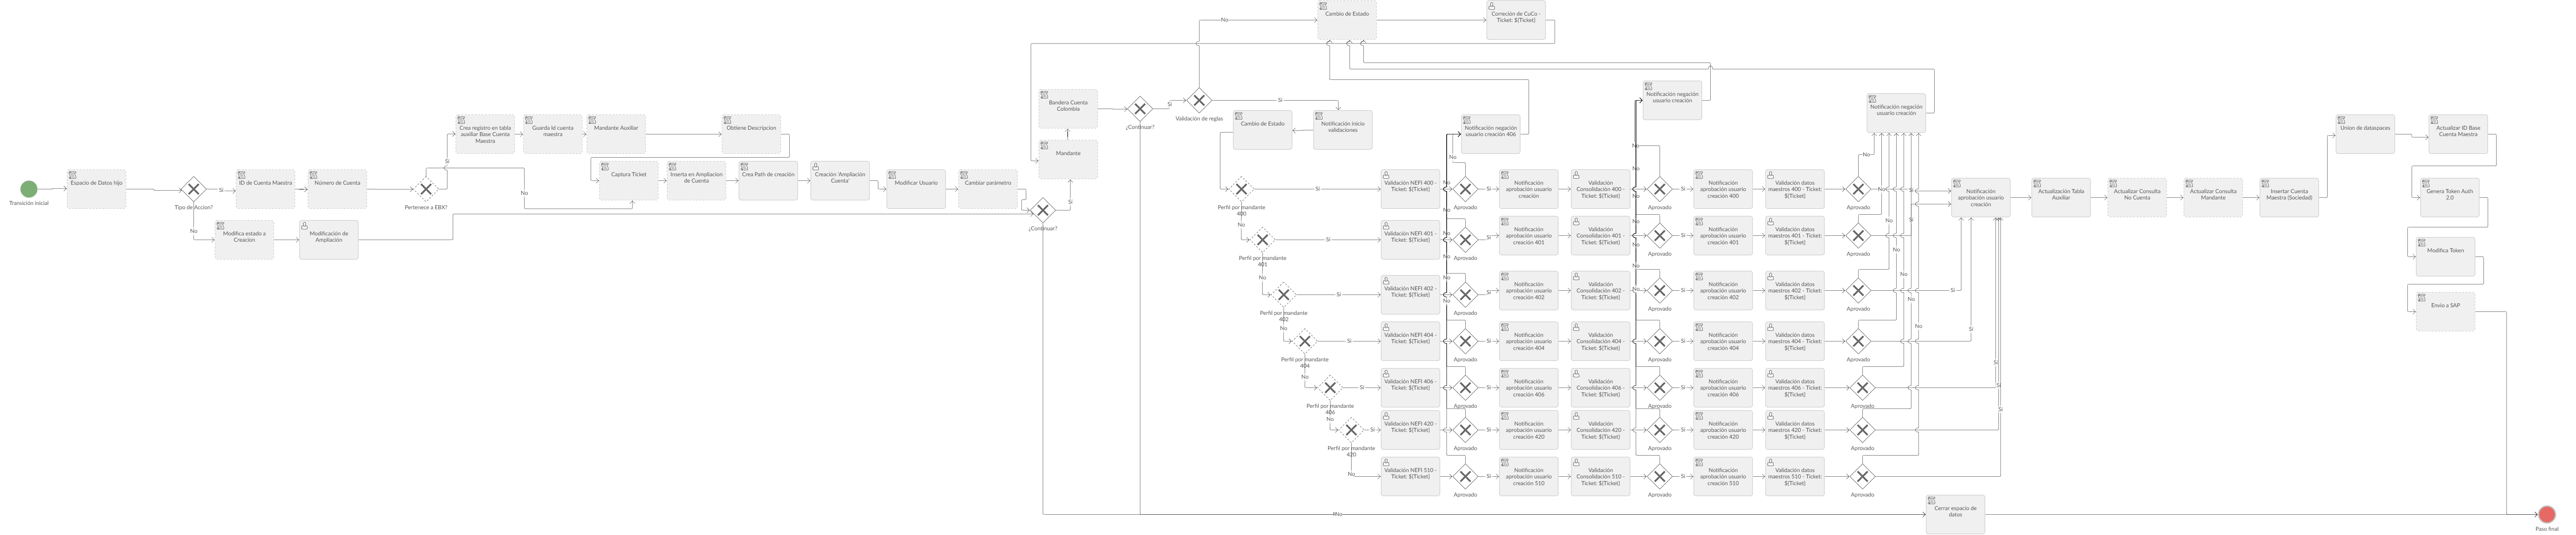
\includegraphics[width=0.8\textwidth]{WorkflowsDashboard/ImgWF/WF06.png}
    \caption{Workflow: Ampliación V2}
\end{figure}

[CuCo] Modificación/Bloqueo (nivel PUC) V2

Flujo de trabajo encargado de realizar el proceso de Modificación/Bloqueo de una cuenta contable. El proceso cuenta con las validaciones necesarias por cada rol utilizado, además incluye la petición de modificación a SAP dentro el proceso.

\begin{figure}[H]
    \centering
    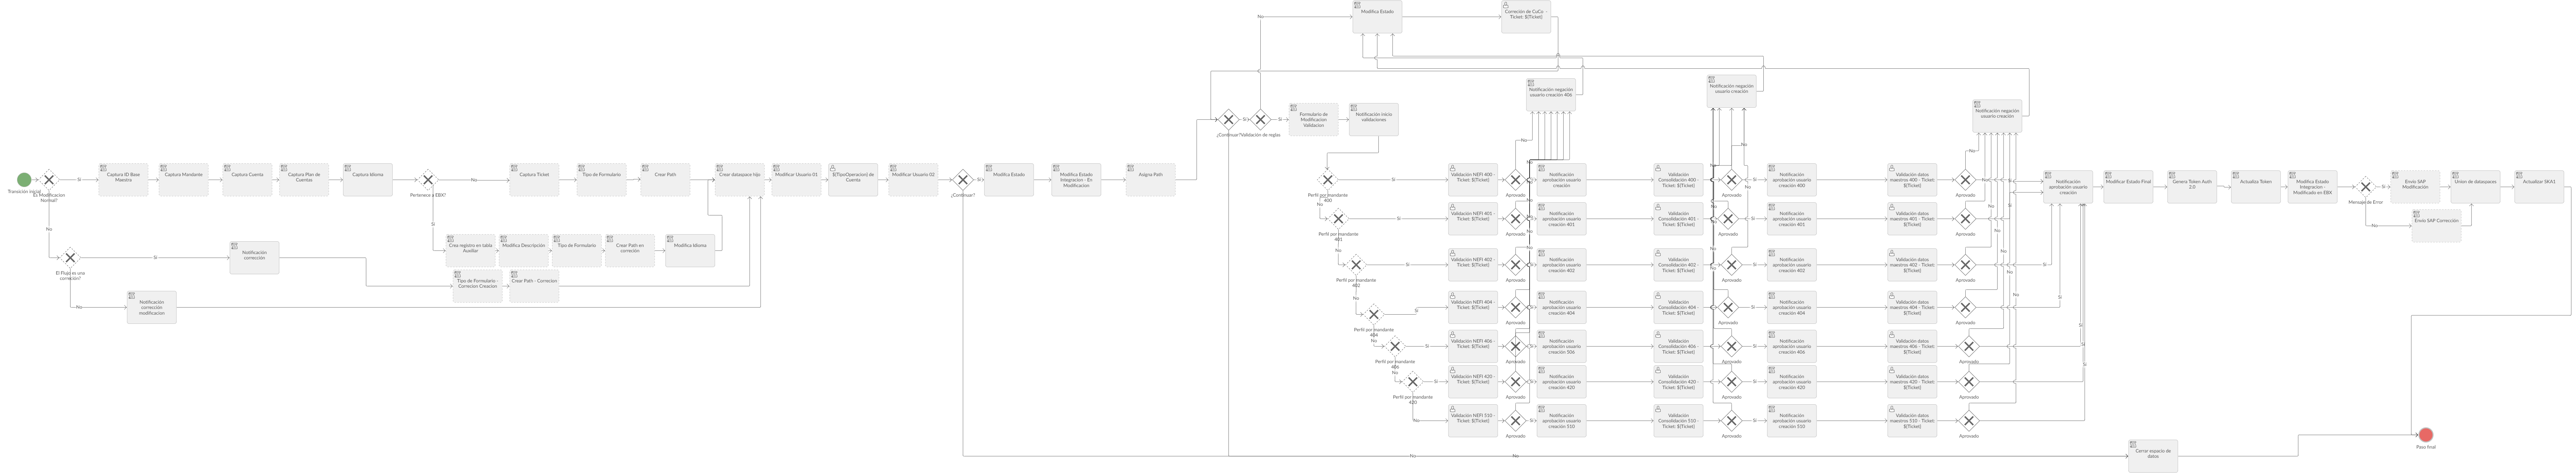
\includegraphics[width=0.8\textwidth]{WorkflowsDashboard/ImgWF/WF07.png}
    \caption{Workflow: Modificación/Bloqueo (nivel PUC) V2}
\end{figure}

[CuCo] Modificación/Bloqueo Expansión de Cuenta V2

Flujo de trabajo encargado de realizar el proceso de Modificación/Bloqueo de una cuenta contable ampliada. El proceso cuenta con las validaciones necesarias por cada rol utilizado, además incluye la petición de modificación a SAP dentro el proceso.

\begin{figure}[H]
    \centering
    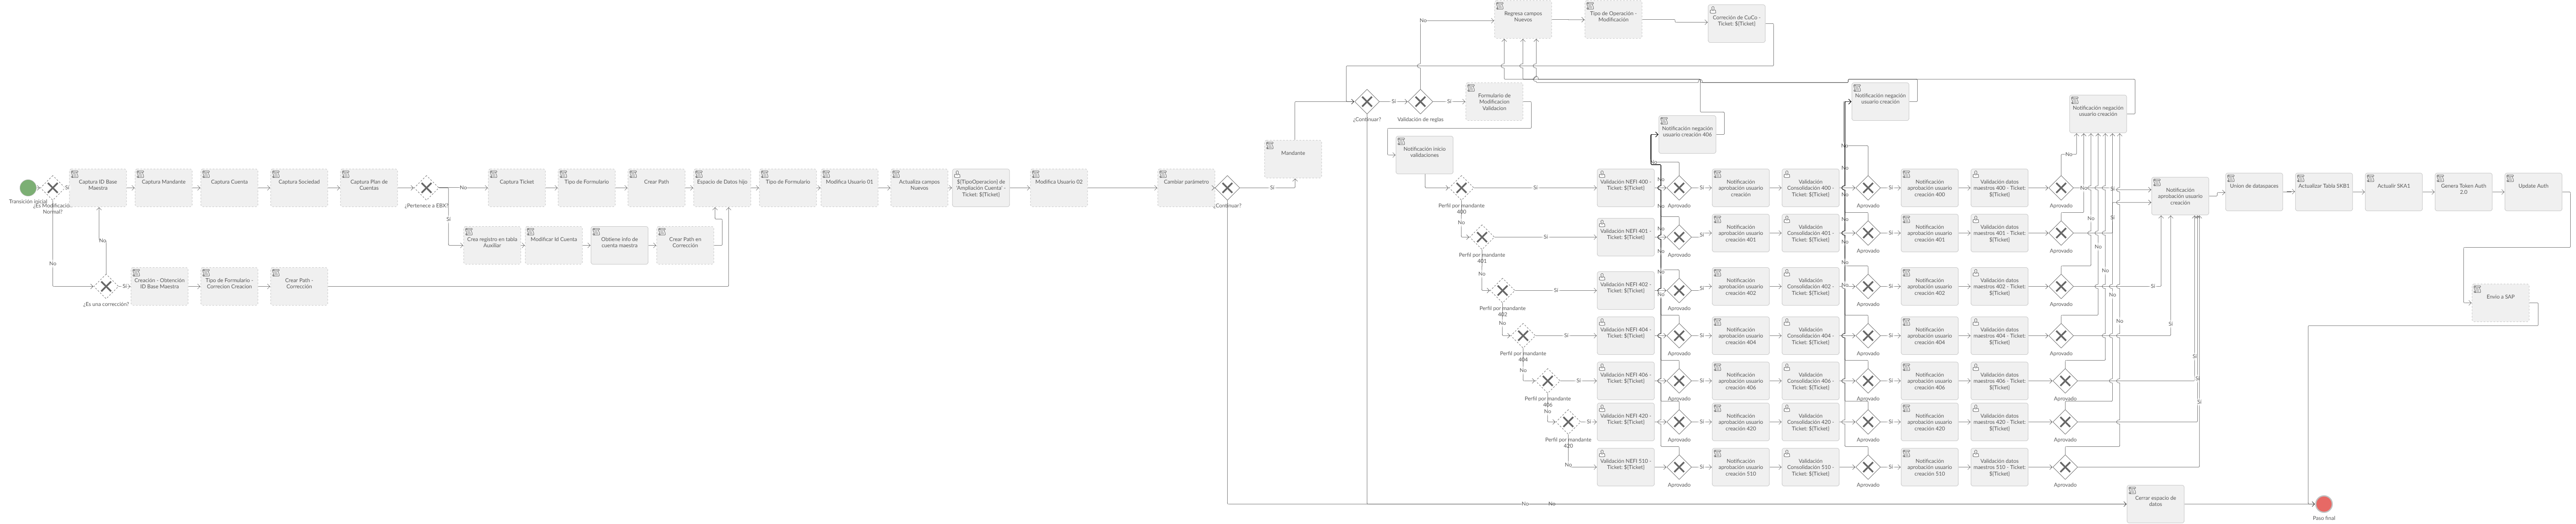
\includegraphics[width=0.8\textwidth]{WorkflowsDashboard/ImgWF/WF08.png}
    \caption{Workflow: Modificación/Bloqueo Expansión de Cuenta V2}
\end{figure}

[CuCo] Creación Multimandante V2

Flujo de trabajo encargado de realizar el proceso de creación de una cuenta contable haciendo uso de todos los mandantes del dominio, además de catálogos externos para facilitar su creación. Dentro del proceso se hace uso de diversos roles para la creación y revisión de la creación. Además, incluye el envío de dicha cuenta a SAP para la creación de su lado.

\begin{figure}[H]
    \centering
    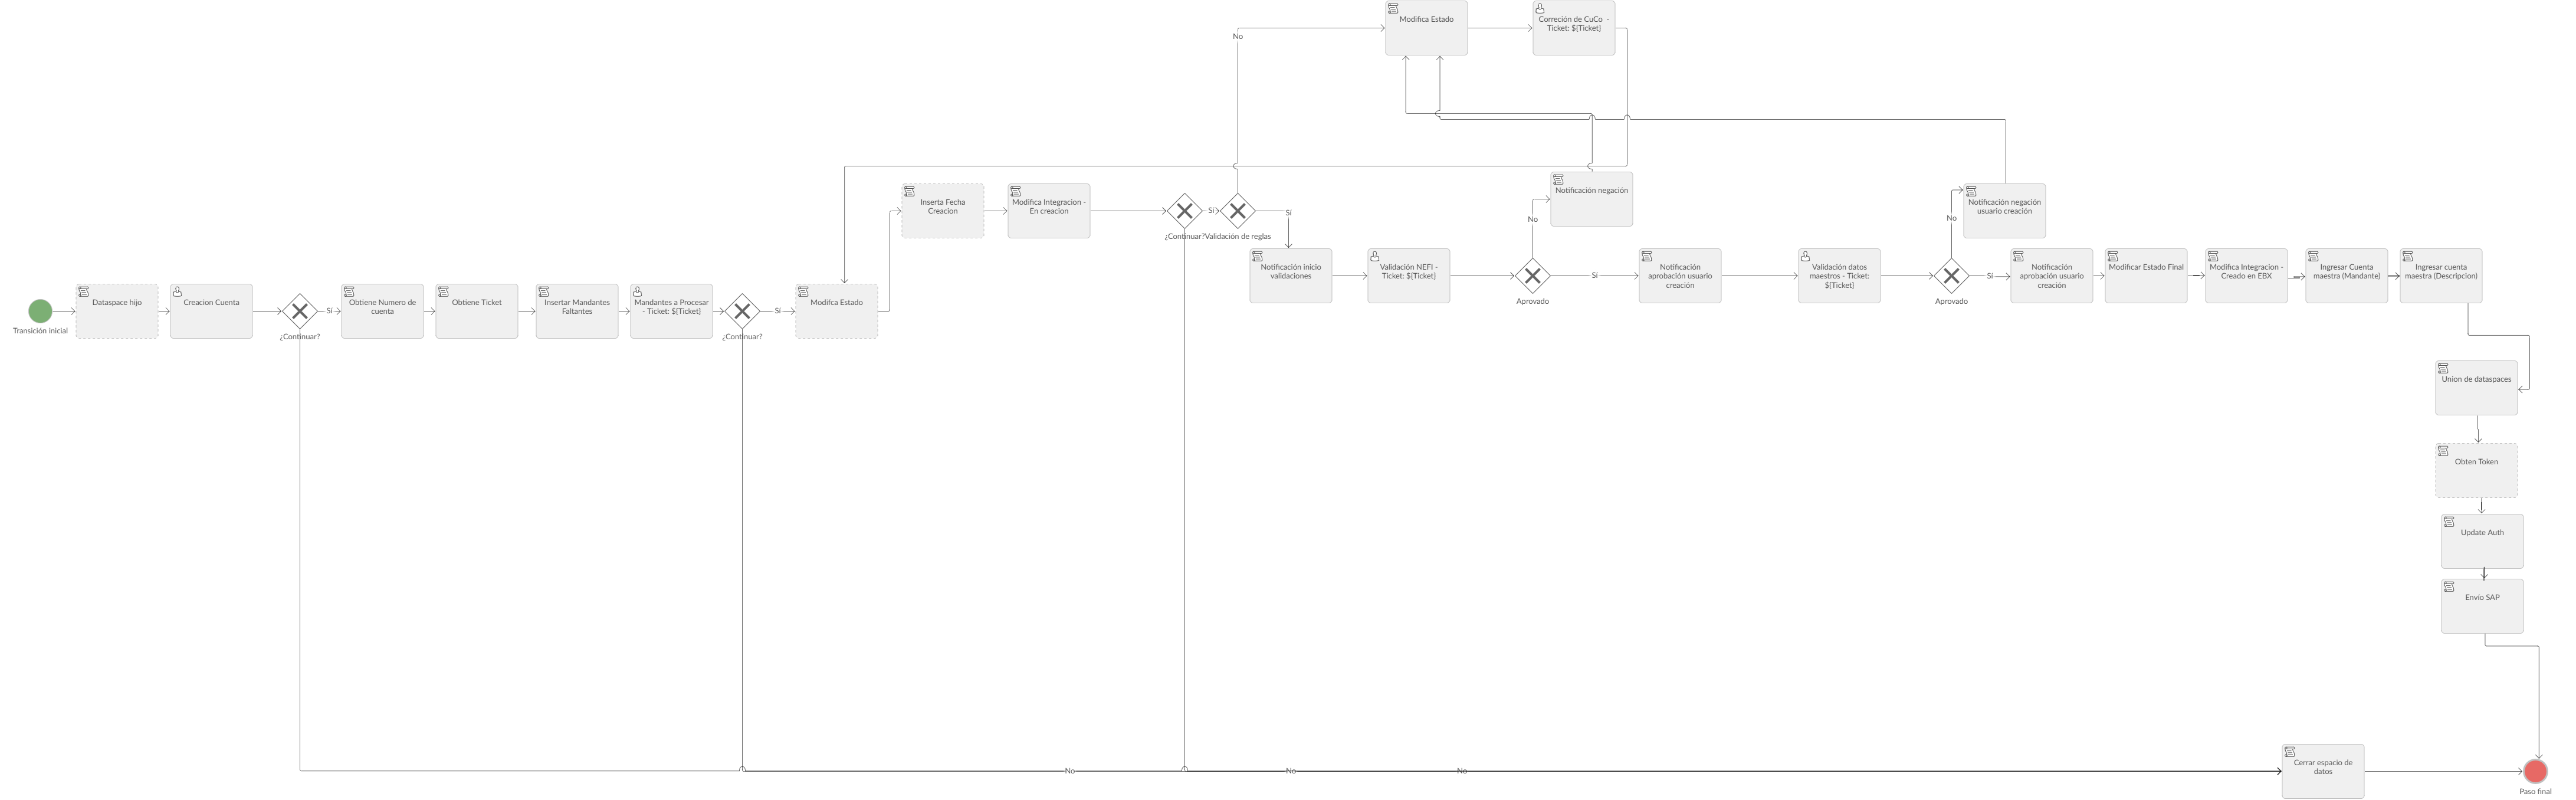
\includegraphics[width=0.8\textwidth]{WorkflowsDashboard/ImgWF/WF09.png}
    \caption{Workflow: Creación Multimandante V2}
\end{figure}

[CuCo] Modificación Multimandante (Nivel PUC) V2

Flujo de trabajo encargado de realizar el proceso de Modificación/Bloqueo de una cuenta contable. El proceso cuenta con las validaciones necesarias por cada rol utilizado; además incluye la petición de modificación a SAP dentro el proceso.

\begin{figure}[H]
    \centering
    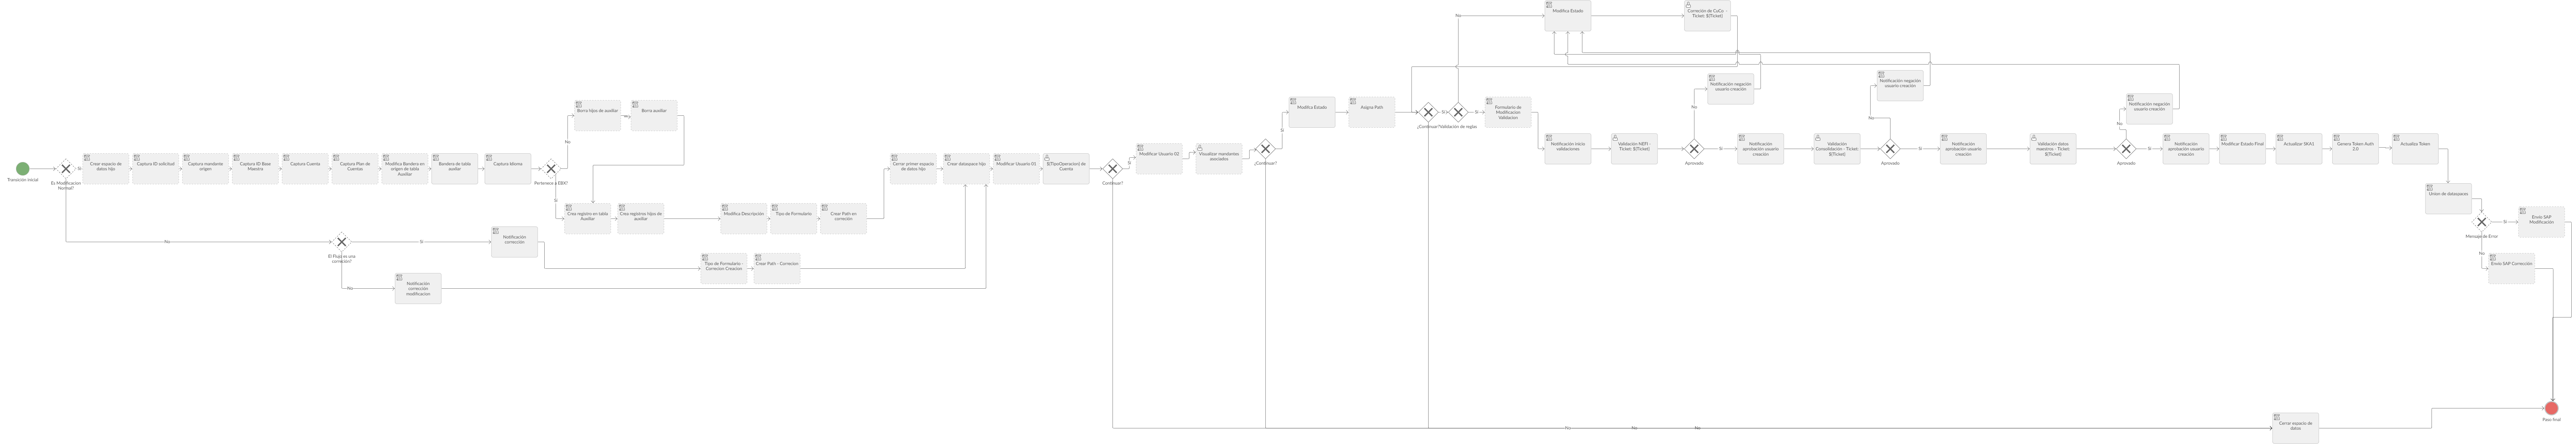
\includegraphics[width=0.8\textwidth]{WorkflowsDashboard/ImgWF/WF10.png}
    \caption{Workflow: Modificación Multimandante (Nivel PUC) V2}
\end{figure}

[CuCo] Modificación/Bloqueo Multi sociedad V2

Flujo de trabajo encargado de realizar el proceso de Modificación/Bloqueo de una cuenta contable ampliada. El proceso cuenta con las validaciones necesarias por cada rol utilizado; además incluye la petición de modificación a SAP dentro el proceso.

\begin{figure}[H]
    \centering
    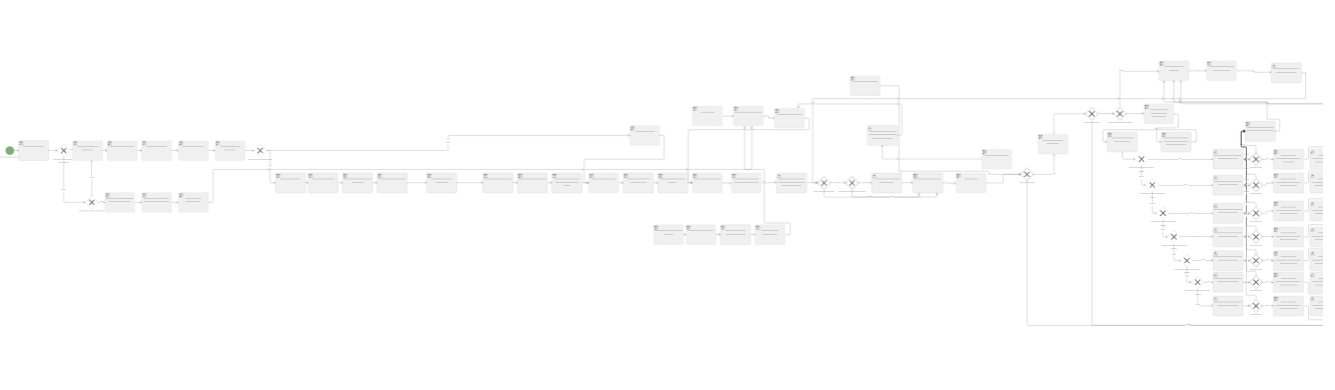
\includegraphics[width=0.8\textwidth]{WorkflowsDashboard/ImgWF/WF11.png}
    \caption{Workflow: Modificación/Bloqueo Multi sociedad V2}
\end{figure}

[CuCo] Notificación Integración SAP - Solace

Flujo de trabajo encargado de mandar una notificación por correo electrónico, al solicitante de la operación, el resultado final de la misma de acuerdo a su impacto en SAP; siempre y cuando haya sido una operación exitosa. 

\begin{figure}[H]
    \centering
    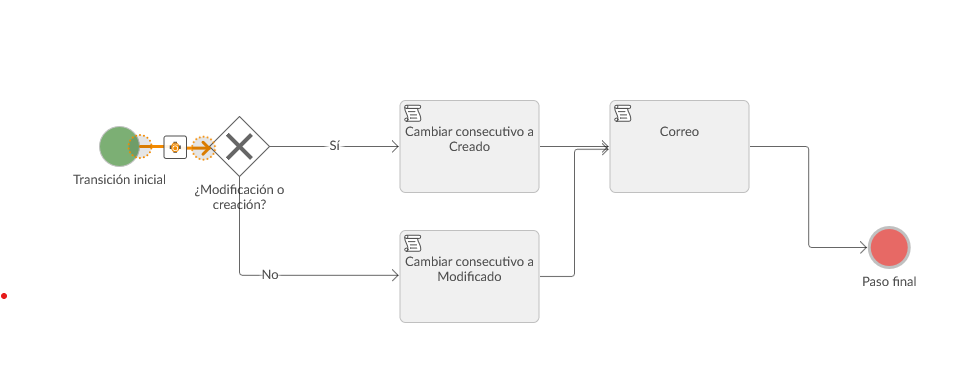
\includegraphics[width=0.8\textwidth]{WorkflowsDashboard/ImgWF/WF12.png}
    \caption{Workflow: Notificación Integración SAP - Solace}
\end{figure}

[CuCo] Reglas de BackEnd V2

Flujo de trabajo que ejecuta las reglas de calidad desarrolladas. Se ejecuta de un módulo a otro por lo cual se ordena por nivel de prioridad.

\begin{figure}[H]
    \centering
    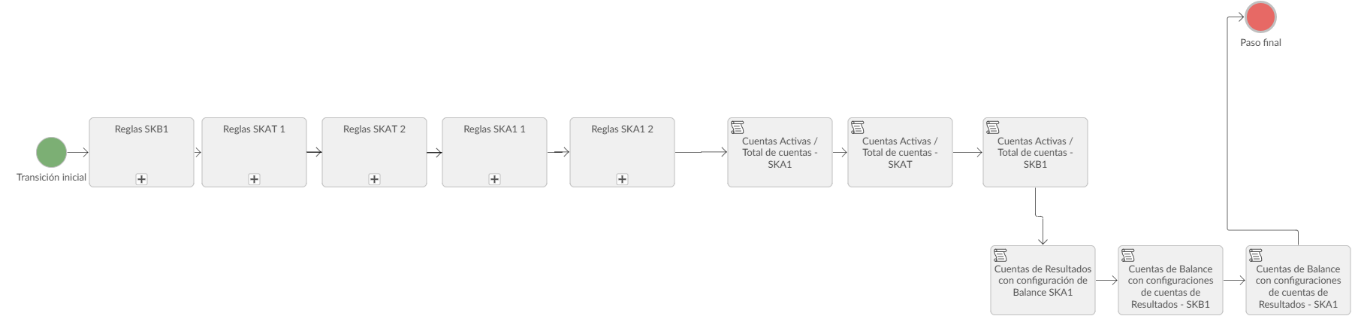
\includegraphics[width=0.8\textwidth]{WorkflowsDashboard/ImgWF/WF13.png}
    \caption{Workflow: Reglas de BackEnd V2}
\end{figure}

%% ############### CARGA MASIVA ###########

[CuCo] Carga Masiva - Nivel PUC V2

Flujo de trabajo que ejecuta el proceso de carga masiva creación, modificación y bloqueo a nivel PUC. 

\begin{figure}[H]
    \centering
    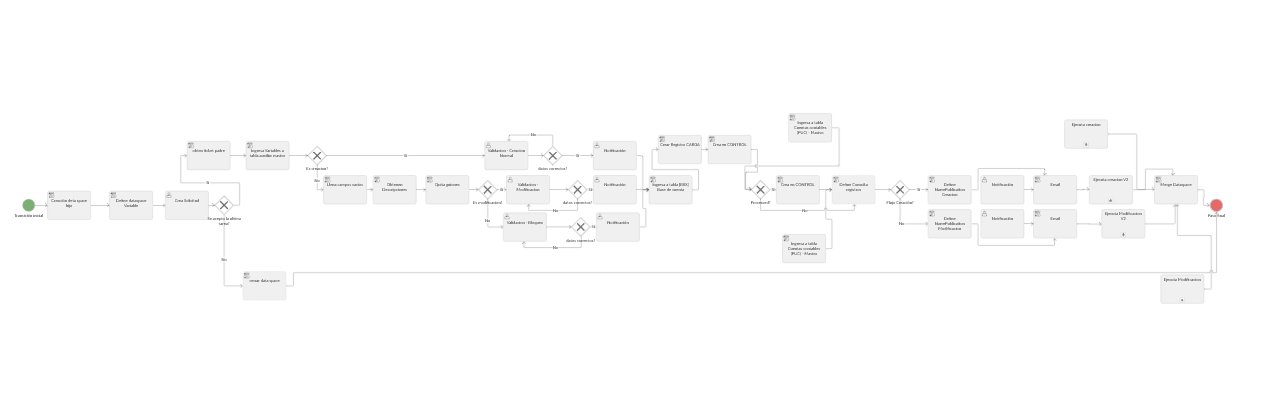
\includegraphics[width=0.8\textwidth]{WorkflowsDashboard/ImgWFMasivo/WFM01.png}
    \caption{Workflow: Carga Masiva - Nivel PUC V2}
\end{figure}

[CuCo] Carga Masiva - Nivel Sociedad V2

Flujo de trabajo que ejecuta el proceso de carga masiva creación, modificación y bloqueo a nivel sociedad.

\begin{figure}[H]
    \centering
    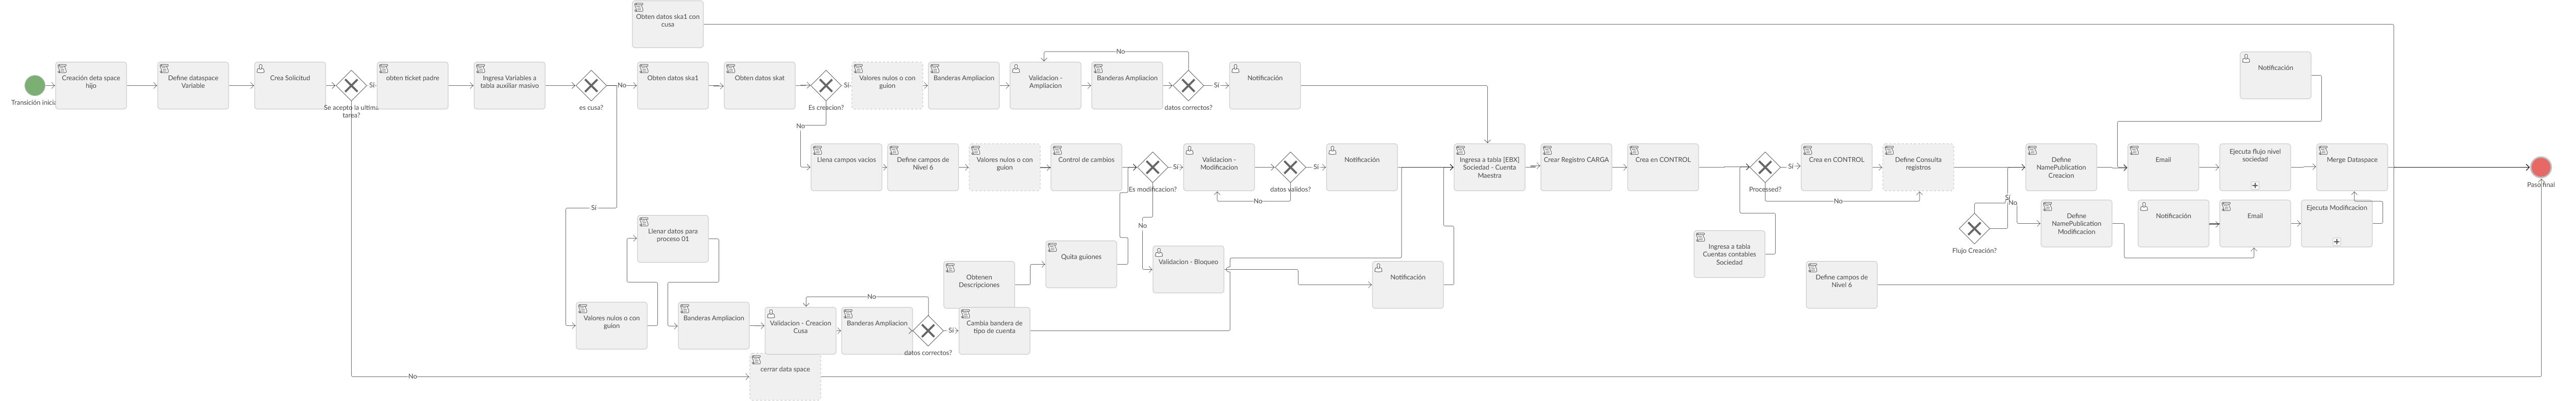
\includegraphics[width=0.8\textwidth]{WorkflowsDashboard/ImgWFMasivo/WFM02.png}
    \caption{Workflow: Carga Masiva - Nivel Sociedad V2}
\end{figure}
%% ############# MASIVOS INDIVIDUALES

[CuCo - Masivo - V2] Creación - Carga Masiva V2

Flujo de trabajo que ejecuta proceso e inicializa validaciones de carga masiva de creación a nivel PUC 

\begin{figure}[H]
    \centering
    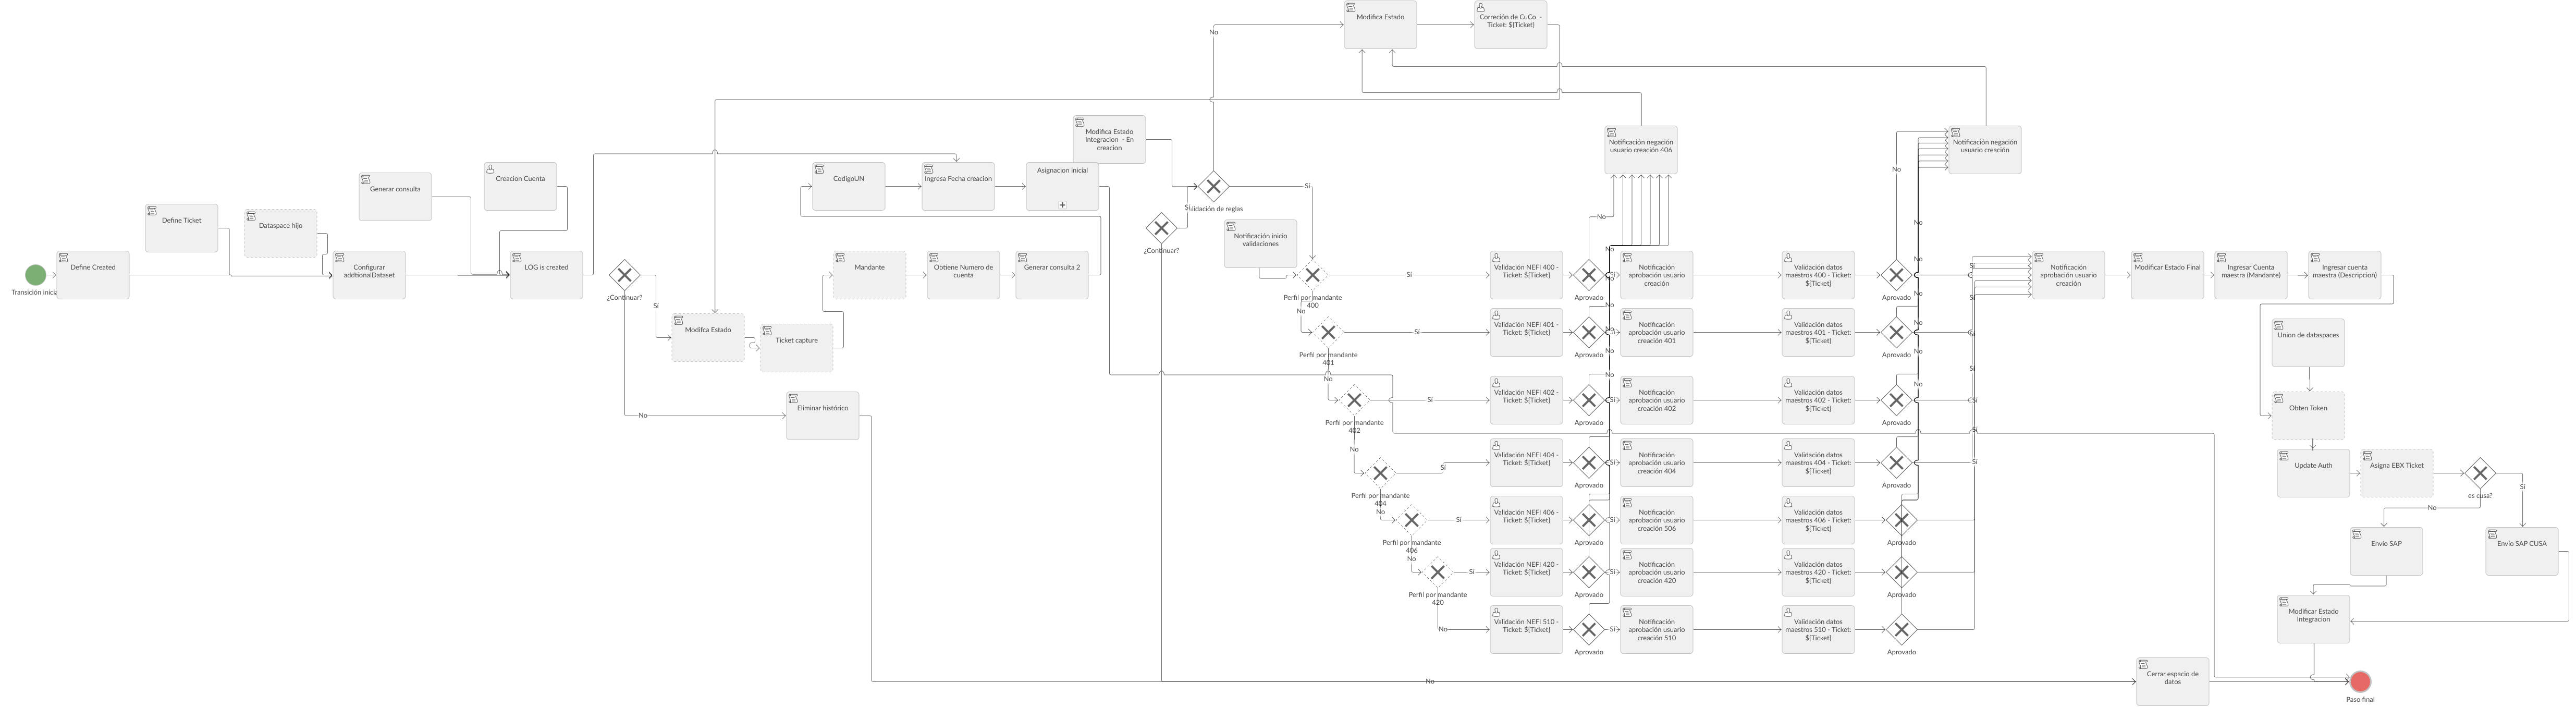
\includegraphics[width=0.8\textwidth]{WorkflowsDashboard/ImgWFMasivo/CreacionMasivaPUC.png}
    \caption{Workflow: [CuCo - Masivo - V2] Creación PUC - Carga Masiva V2}
\end{figure}


[CuCo - Masivo - V2] Modificación PUC - Carga Masiva V2

Flujo de trabajo que ejecuta proceso e inicializa validaciones de carga masiva de modificación/ bloqueo/ desbloqueo a nivel PUC 

\begin{figure}[H]
    \centering
    
\includegraphics[width=0.8\textwidth]{WorkflowsDashboard/ImgWFMasivo/ModificacionMasivaPUC.png}
    \caption{Workflow: [CuCo - Masivo - V2] Modificación PUC - Carga Masiva V2}
\end{figure}

[CuCo - Masivo - V2] Ampliación/Modificación - Carga Masiva V2

Flujo de trabajo que ejecuta proceso e inicializa validaciones de carga masiva a nivel sociedad

\begin{figure}[H]
    \centering
    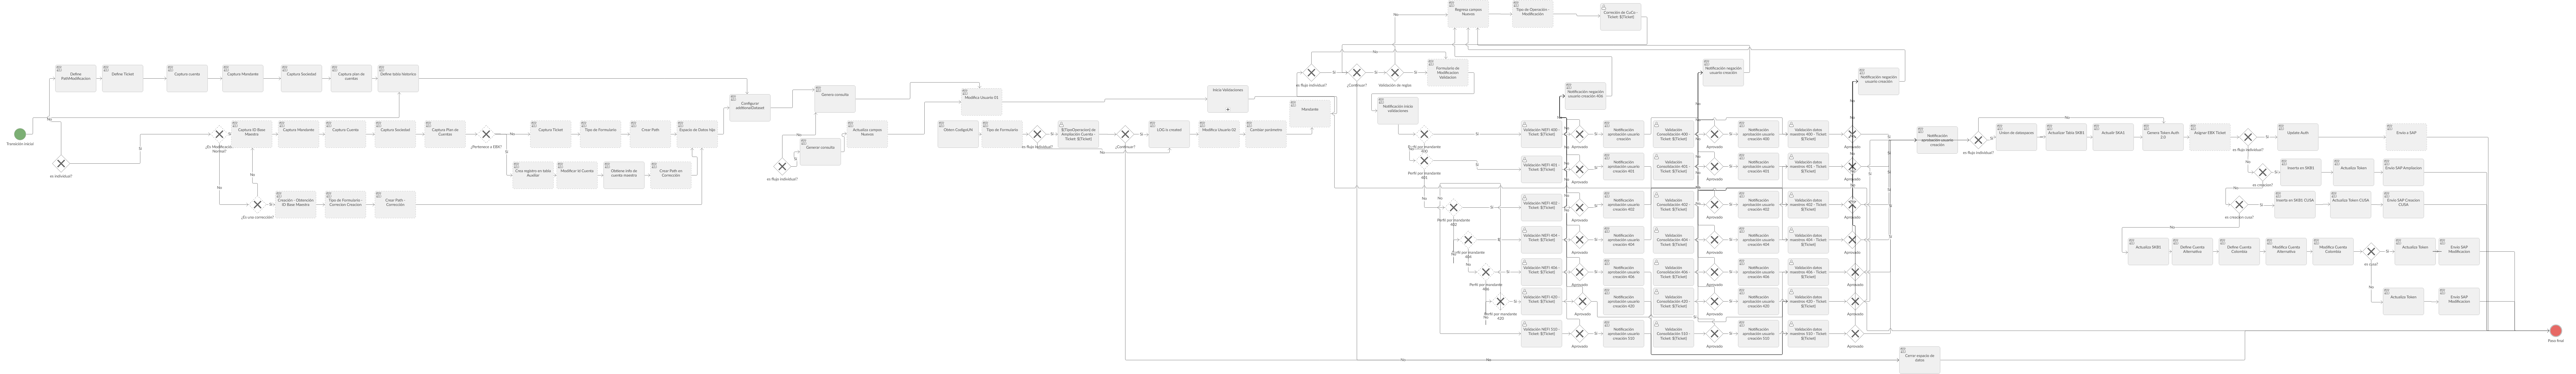
\includegraphics[width=0.8\textwidth]{WorkflowsDashboard/ImgWFMasivo/AmpModMasivo.png}
    \caption{Workflow: [CuCo - Masivo - V2] Ampliación/Modificación - Carga Masiva V2}
\end{figure}


%% ####### inicializadores generales

[CuCo - Masivo - V2] Asignación Inicial - Carga Masiva V2

Flujo de trabajo que ejecuta inicializa las precarga de datos en las tablas auxiliares de carga masiva.

\begin{figure}[H]
    \centering
    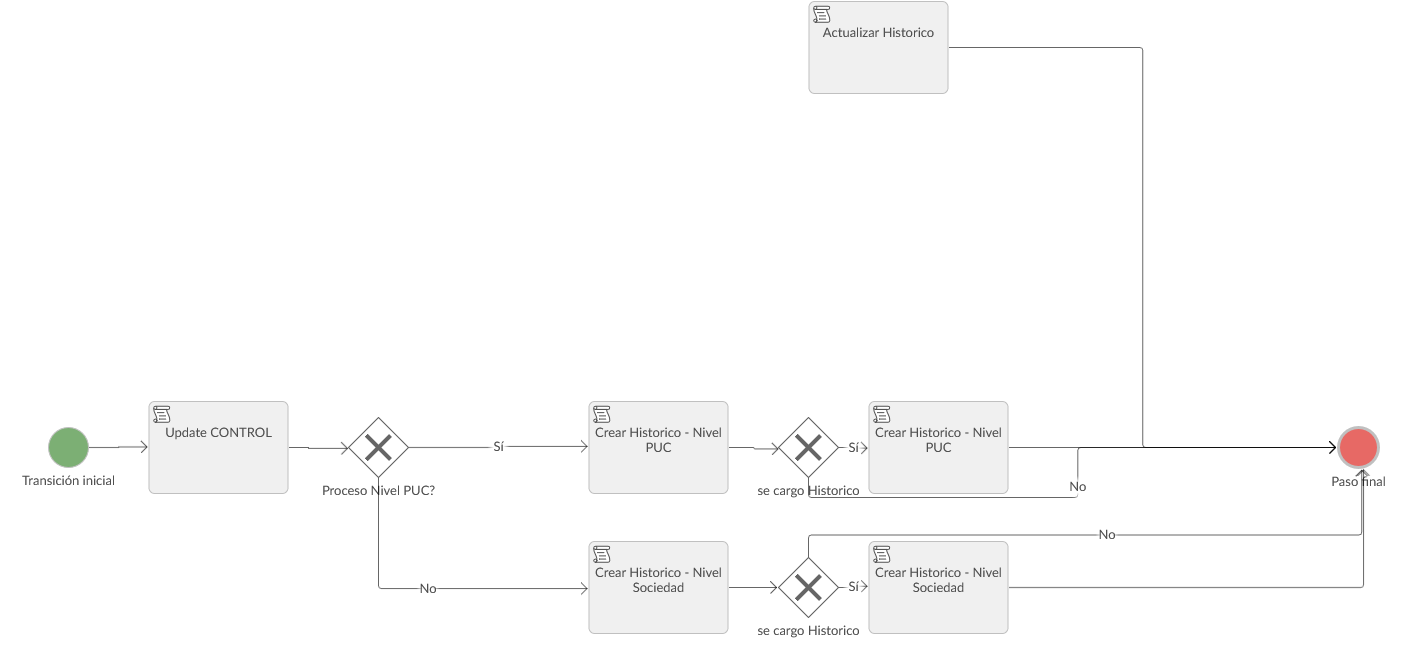
\includegraphics[width=0.8\textwidth]{WorkflowsDashboard/ImgWFMasivo/CuCoMasivoAsignacionInicial.png}
    \caption{Workflow: [CuCo - Masivo - V2] Asignación Inicial - Carga Masiva V2}
\end{figure}


[CuCo - Masivo - V2] Envió de Correos - Carga Masiva V2

Flujo de trabajo que ejecuta el envió de correos por bloques de mandantes a los validadores en cuestión de paso actual.

\begin{figure}[H]
    \centering
    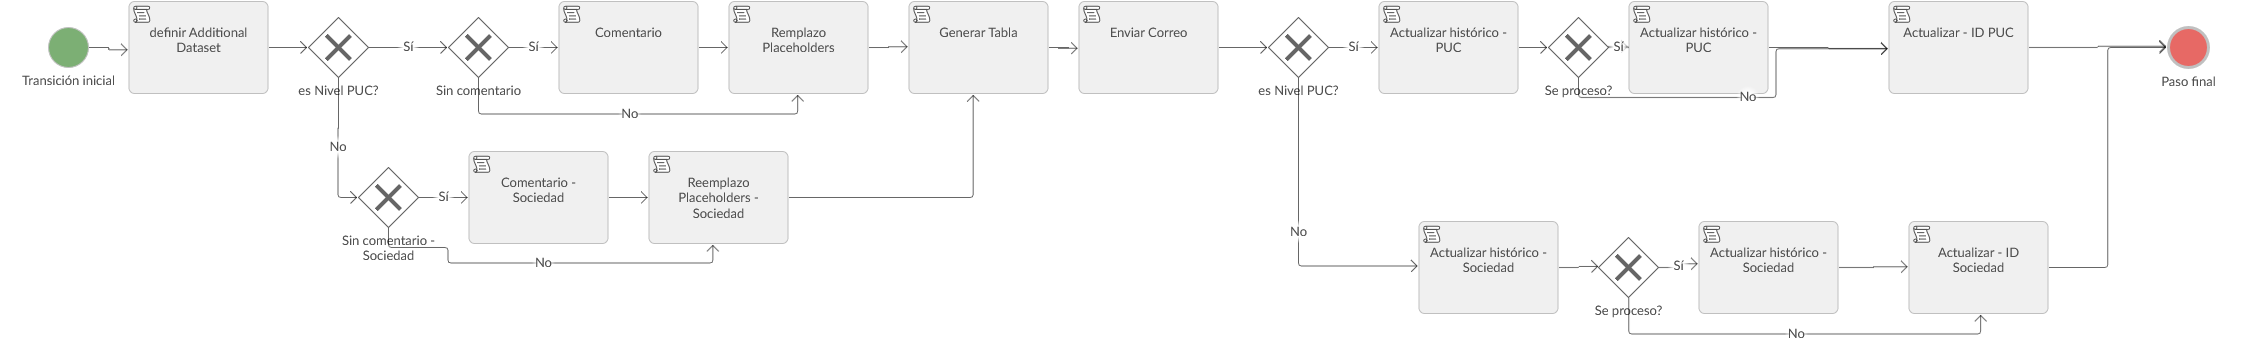
\includegraphics[width=0.8\textwidth]{WorkflowsDashboard/ImgWFMasivo/CuCoMasivoMailTable.png}
    \caption{Workflow: [CuCo - Masivo - V2] Envió de Correos - Carga Masiva V2}
\end{figure}

[CuCo - Masivo - V2] Validación - Carga Masiva V2

Flujo de trabajo que ejecuta la validación del registro individual y en las tablas de gestión de la carga masiva.

\begin{figure}[H]
    \centering
    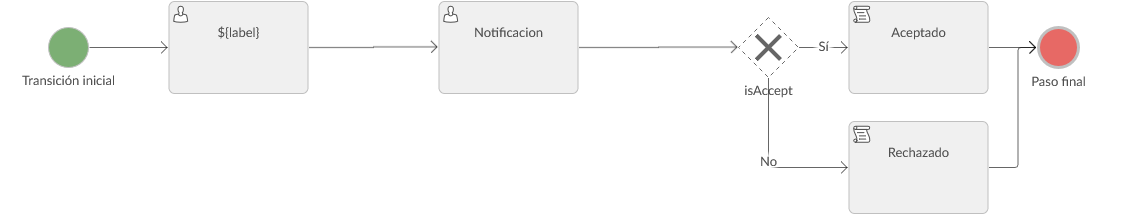
\includegraphics[width=0.8\textwidth]{WorkflowsDashboard/ImgWFMasivo/CuCoMasivoValidacion.png}
    \caption{Workflow: [CuCo - Masivo - V2] Validación - Carga Masiva V2}
\end{figure}

[CuCo - Masivo - V2] Validación Solicitante- Carga Masiva V2

Flujo de trabajo que se ejecuta cuando es negado un bloque de registros dentro el proceso, este se le asigna al solicitante para su validación.

\begin{figure}[H]
    \centering
    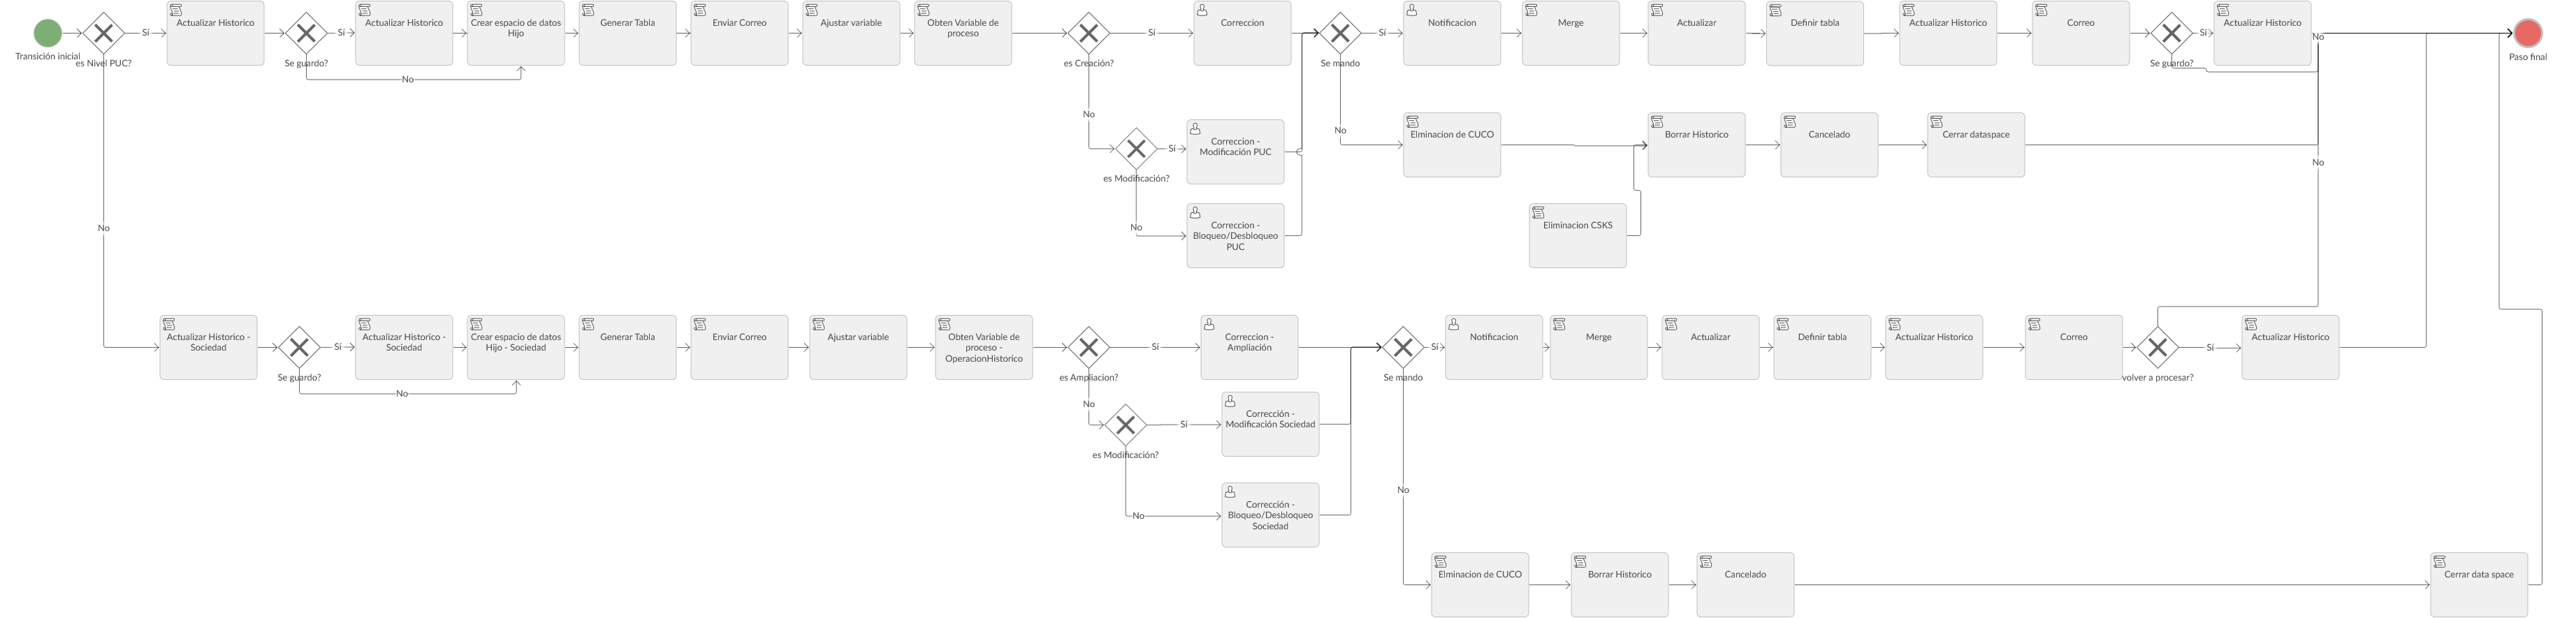
\includegraphics[width=0.8\textwidth]{WorkflowsDashboard/ImgWFMasivo/CuCoValidacionSolicitante.png}
    \caption{Workflow: [CuCo - Masivo - V2] Validación Solicitante - Carga Masiva V2}
\end{figure}


[CuCo - Masivo - V2] Envió SAP Unidades - Carga Masiva V2

Flujo de trabajo que se genera las solicitudes de integración por bloques de unidades de negocio, además de contener las actualizaciones finales a los registros en las tablas de gestión.

\begin{figure}[H]
    \centering
    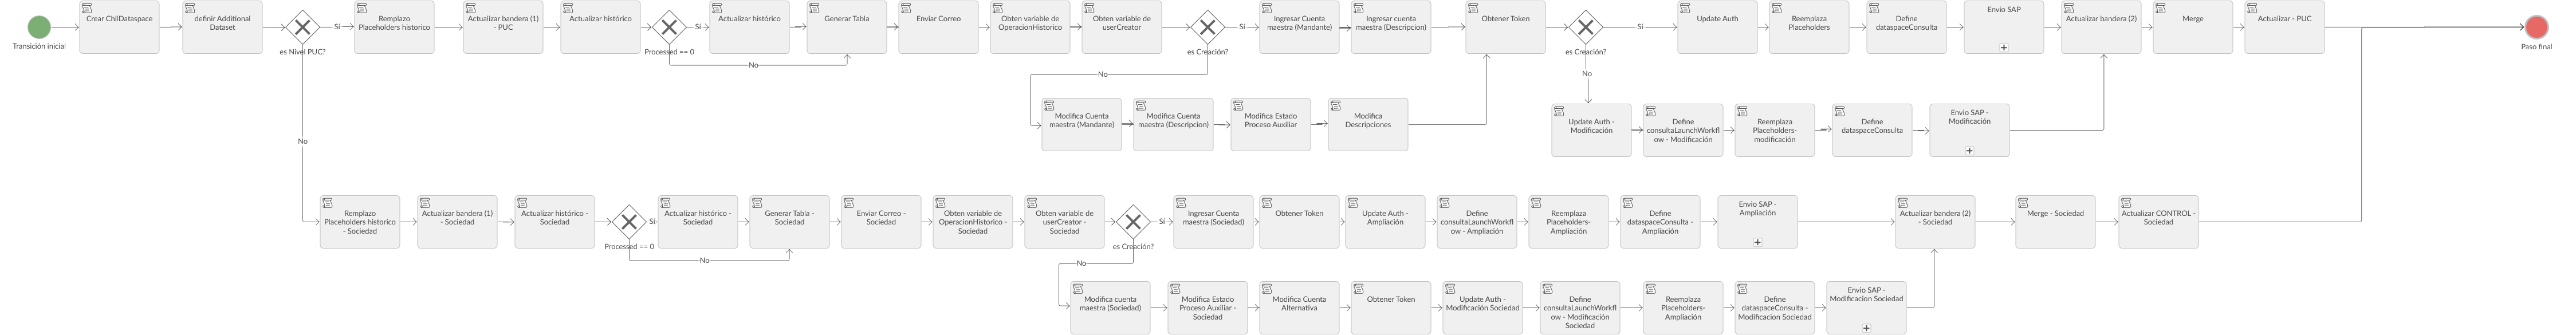
\includegraphics[width=0.8\textwidth]{WorkflowsDashboard/ImgWFMasivo/CuCoEnvioSAPUnidades.png}
    \caption{Workflow: [CuCo - Masivo - V2] Envió SAP Unidades - Carga Masiva V2}
\end{figure}


\begin{quote}
  \textbf{Nota:} Para mejor información técnica de cada Workflow y script se puede consultar los anexos de:
  \begin{itemize}
    \item Memoria Técnica finanzas – Scripts Creación/Ampliación
    \item Memoria Técnica finanzas – Scripts Modificación
  \end{itemize}
\end{quote}



